\documentclass{beamer}
\usepackage{ArmenianSlides}

\begin{document}

\title[ChainOfResponsibility]{Նախագծման Ձևանմուշներ։ ChainOfResponsibility}
\author[Հրաչյա Թանդիլյան\copyright]{Հրաչյա Թանդիլյան}
\date{2020}

%-------------------------------------------------------------------------------------------------
\begin{frame}
\titlepage
\end{frame}
%-------------------------------------------------------------------------------------------------

\section{Նպատակը}
%-------------------------------------------------------------------------------------------------
\begin{frame}\frametitle{ChainOfResponsibility}
\begin{block}{Նպատակը}
    Խուսափել հարցում ուղարկողին հարցումը ստացողին կապելուց` հնարավորություն
    ընձեռելով մեկից ավել օբյեկտների սպասարկել այն: \\
    \vspace{0.5cm}
    Կառուցել ստացող օբյեկտների շղթա և հարցումը այդ շղթայով փոխանցել քանի դեռ
    ինչ-որ օբյեկտ այն չմշակի:
\end{block}
\vfill
Նաև հայտնի է որպես
\begin{itemize}
    \item Այլ լայնորեն կիրառվող անուներ չկան:
\end{itemize}
\end{frame}
%-------------------------------------------------------------------------------------------------

\subsection{Մոտիվացիան}
%-------------------------------------------------------------------------------------------------
\begin{frame}\frametitle{Մոտիվացիան}
\begin{center}
    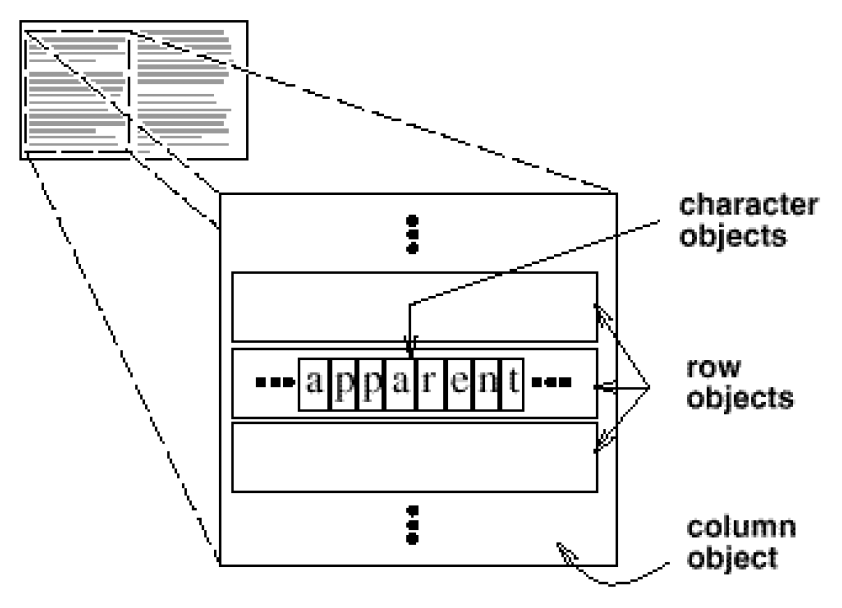
\includegraphics[scale=0.4]{motivation1.png}
\end{center}
\end{frame}
%-------------------------------------------------------------------------------------------------

%-------------------------------------------------------------------------------------------------
\begin{frame}\frametitle{Մոտիվացիան}
\begin{center}
    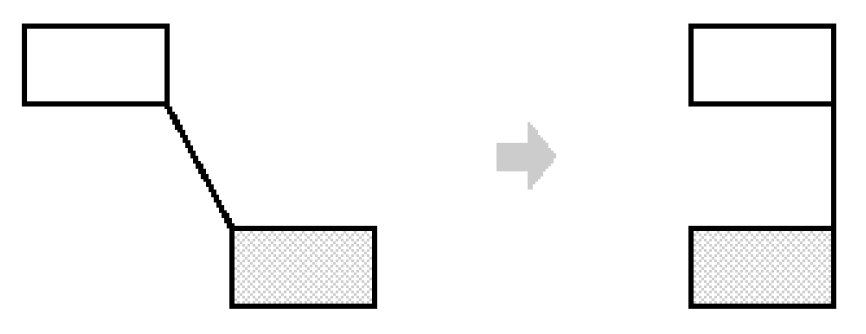
\includegraphics[scale=0.4]{motivation2.png}
\end{center}
\end{frame}
%-------------------------------------------------------------------------------------------------

%-------------------------------------------------------------------------------------------------
\begin{frame}\frametitle{Մոտիվացիան}
\begin{center}
    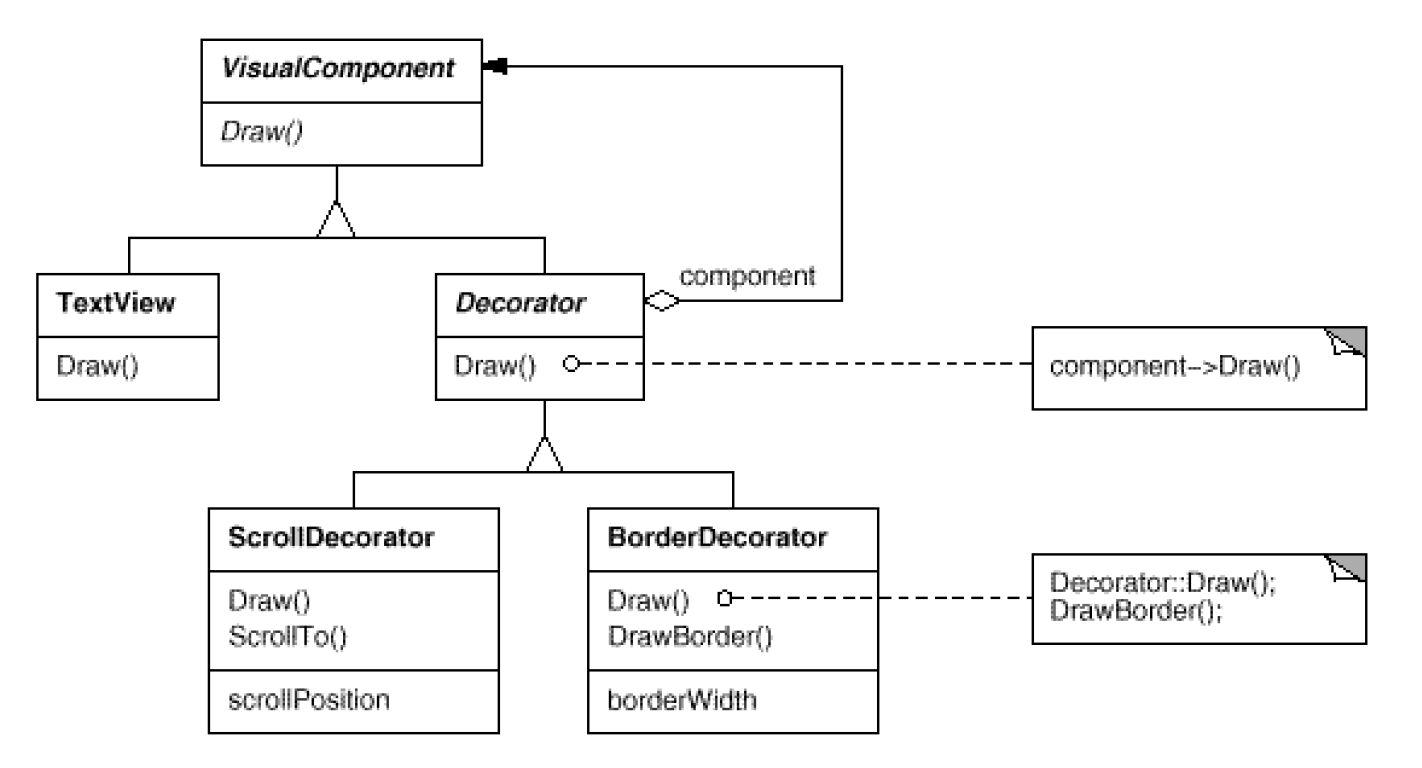
\includegraphics[scale=0.4]{motivation3.png}
\end{center}
\end{frame}
%-------------------------------------------------------------------------------------------------

\subsection{Կիրառելիությունը}
%-------------------------------------------------------------------------------------------------
\begin{frame}\frametitle{Կիրառելիությունը}
Այս Ն.Ձ. պետք է օգտագործել երբ.
\vfill
\begin{enumerate}
    \scriptsize
    \item Մեկից ավելի օբյեկտներ կարող են սպասարկել հարցումը, բայց կոնկրետ
    սպասարկողը նախապես հայտնի չէ: Անհրաժեշտ է սպասարկողի պարզումը
    իրականացնել ավտոմատ կերպով: \pause \vfill
    \item Անհրաժեշտ է հարցում տալ մի քանի օբյեկտներից մեկին առանց բացահայտ
    կերպով ստացողին նշելու: \pause \vfill
    \item Հարցումներ սպասարկող օբյեկտների բազմությունը պետք է նշվի (սահմանվի)
    դինամիկ կերպով:
\end{enumerate}
\end{frame}
%-------------------------------------------------------------------------------------------------

\section{Կառուցվածքը}
%-------------------------------------------------------------------------------------------------
\begin{frame}\frametitle{Կառուցվածքը}
\begin{center}
    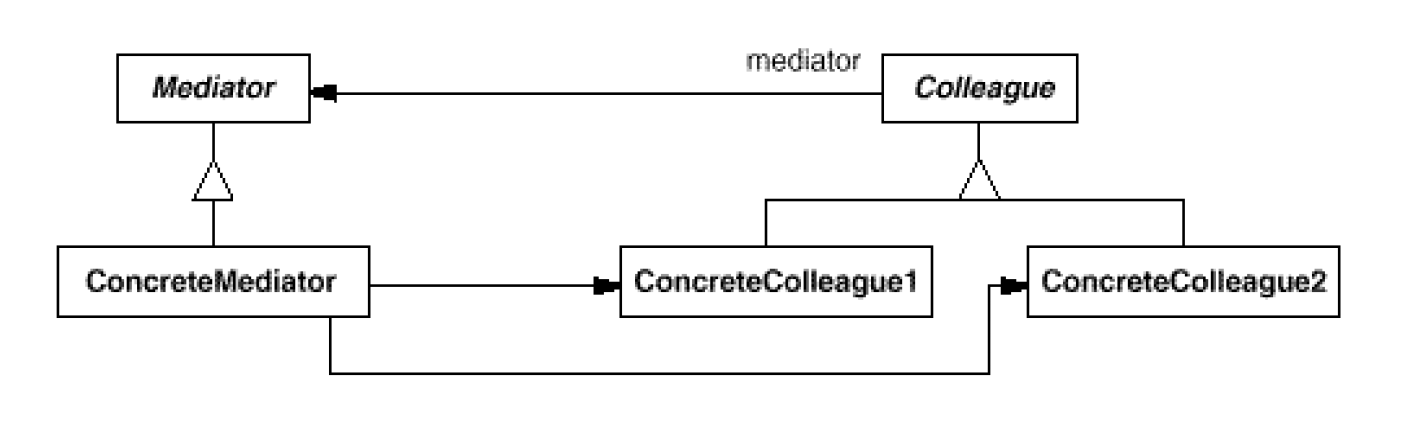
\includegraphics[scale=0.4]{structure1.png}
    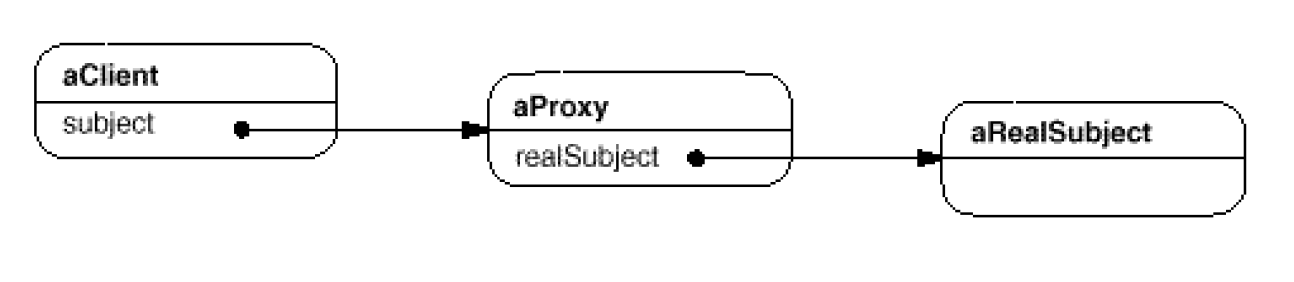
\includegraphics[scale=0.4]{structure2.png}
\end{center}
\end{frame}
%-------------------------------------------------------------------------------------------------

\subsection{Հետևանքները}
%-------------------------------------------------------------------------------------------------
\begin{frame}\frametitle{Հետևանքները}
Այս Ն.Ձ. ունի հետևյալ առավելություններն ու թերությունները.
\vfill
\begin{enumerate}
    \item Նվազեցնում է կապվածությունը: \pause \vfill
    \item Ճկունացնում է օբյեկտներին պատասխանատվության համապատասխանեցումը: \pause \vfill
    \item Ստացողի գոյությունը երաշխավորված չէ:
\end{enumerate}
\end{frame}
%-------------------------------------------------------------------------------------------------

\section{Իրականացումը}
%-------------------------------------------------------------------------------------------------
\begin{frame}\frametitle{Իրականացումը}
\begin{enumerate}
    \item Իրավահաջորդների շղթայի իրականացումը: \vfill
    \item Իրավահաջորդների կապակցումը: \vfill
    \item Հարցումների ներկայացումը:
\end{enumerate}
\end{frame}
%-------------------------------------------------------------------------------------------------

\subsection{Օրինակ}
%-------------------------------------------------------------------------------------------------
\begin{frame}[fragile]\frametitle{Օրինակ}
\begin{english}
\begin{minted}[fontsize=\tiny]{cpp}
class HelpHandler {

public:
    enum Topic {
        NO_HELP_TOPIC = -1, PAPER_ORIENTATION_TOPIC,
        PRINT_TOPIC, APPLICATION_TOPIC
    };

public:
    HelpHandler(HelpHandler* h = 0, Topic t = NO_HELP_TOPIC)
        : successor(h), topic(t) {}

    virtual bool HasHelp() {
        return topic != NO_HELP_TOPIC;
    }
    virtual void HandleHelp() {
        if (successor != 0)  {
            successor->HandleHelp();
        }
    }
    virtual void SetHandler(HelpHandler*, Topic);

private:
    HelpHandler* successor;
    Topic topic;
};
\end{minted}
\end{english}
\end{frame}
%-------------------------------------------------------------------------------------------------

%-------------------------------------------------------------------------------------------------
\begin{frame}[fragile]\frametitle{Օրինակ}
\begin{english}
\begin{minted}{cpp}
class Widget : public HelpHandler {

protected:
    Widget(Widget* p, Topic t = NO_HELP_TOPIC)
        : HelpHandler(p, t), parent(p) {}

private:
    Widget* parent;
};
\end{minted}
\end{english}
\end{frame}
%-------------------------------------------------------------------------------------------------

%-------------------------------------------------------------------------------------------------
\begin{frame}[fragile]\frametitle{Օրինակ}
\begin{english}
\begin{minted}{cpp}
class Button : public Widget {

public:
    Button(Widget* w, Topic t = NO_HELP_TOPIC)
        : Widget(w, t) {}

    virtual void HandleHelp() {
        if (!HasHelp()) {
            HelpHandler::HandleHelp();
        }
        // Offer help on the button
    }
    // Widget operations that Button overrides
};
\end{minted}
\end{english}
\end{frame}
%-------------------------------------------------------------------------------------------------

%-------------------------------------------------------------------------------------------------
\begin{frame}[fragile]\frametitle{Օրինակ}
\begin{english}
\begin{minted}{cpp}
class Dialog : public Widget {

public:
    Dialog(HelpHandler* h, Topic t = NO_HELP_TOPIC)
        : Widget(0) {
        SetHandler(h, t);
    }
    virtual void HandleHelp() {
        if (!HasHelp()) {
            HelpHandler::HandleHelp();
        }
        // Offer help on the dialog
    }
    // Widget operations that Dialog overrides
};
\end{minted}
\end{english}
\end{frame}
%-------------------------------------------------------------------------------------------------

%-------------------------------------------------------------------------------------------------
\begin{frame}[fragile]\frametitle{Օրինակ}
\begin{english}
\begin{minted}{cpp}
class Application : public HelpHandler {

public:
    Application(Topic t) : HelpHandler(0, t) {}

    virtual void HandleHelp() {
        // Show a list of help topics
    }
    // Application-specific operations
};
\end{minted}
\end{english}
\end{frame}
%-------------------------------------------------------------------------------------------------

%-------------------------------------------------------------------------------------------------
\begin{frame}[fragile]\frametitle{Օրինակ}
\begin{english}
\begin{minted}{cpp}
Application* application = new Application(APPLICATION_TOPIC);

Dialog* dialog = new Dialog(application, PRINT_TOPIC);

Button* button = new Button(dialog, PAPER_ORIENTATION_TOPIC);

button->HandleHelp();
\end{minted}
\end{english}
\end{frame}
%-------------------------------------------------------------------------------------------------

\section{Առնչվող Ձևանմուշները}
%-------------------------------------------------------------------------------------------------
\begin{frame}\frametitle{Առնչվող Նախագծման Ձևանմուշները}
\begin{itemize}
    \item Composite
\end{itemize}
\end{frame}
%-------------------------------------------------------------------------------------------------

\end{document}
